\subsubsection{Aufbau eines EMI-Filters} \label{subsubsec:emi_filter}
Ein EMI-Filter ist ein lineares Netzwerk aus R, L, C Bauteilen und einem Transformator. Somit besitzten sie eine reziproke Übertragungssymetrie, was eine einfache Berechnungen von verschiedenen Zusammenhängen erlaubt. Einem reziproken Netzwerk ist die Betriebsrichtung gleichgültig.
Die Schaltung \ref{fig:orig_Schaltung} \nameref{fig:orig_Schaltung} zeigt den Filteraufbau, wie er der Aufgabenstellung zu entnehmen ist. Um das Gegentaktrauschen und das Gleichtaktrauschen bestimmen zu können, werden die beiden Schaltungsäquivalente gebildet. 

\begin{figure}[H]
	\centering
	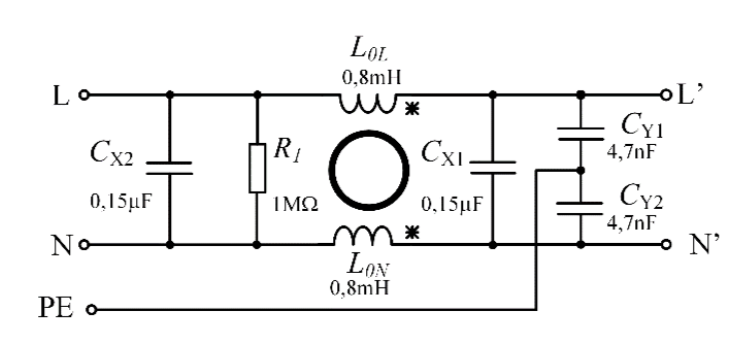
\includegraphics[width = 10cm]{orig_ElectricalCircuit.png}
	\caption{Original Schaltung \cite{aufgabenstellung}}
	\label{fig:orig_Schaltung}
\end{figure}


%TODO Die Schaltungsäquivalenzen müssen aufgeteilt werden und in die jeweiligen subsubsections gekippt werden
%TODO Reziprokzität einfügen
%TODO Allgemein EMI-Filter beschreiben
\subsubsection{2-Tore} \label{subsubsec:emi_filter}

In der Elektrotechnik sind 2-Tore Systeme mit 2 Klemmenpaaren (Tore), die intern aus beliebigen
R (ohmischer Widerstand), L (Induktivität), C (Kapazität) und M(Gegeninduktivität) Komponenten aufgebaut sind. 
Dabei wird ein Tor als Eingang für ein Elektrisches Signal verwendet. Folglich wird bei den Ausgangsklemmen das Ausgangssignal abgegriffen. 
Es wird zwischen aktiv und passiv unterschieden.
Bei aktiven Zweitoren wird die Leistung, die beim Eingang eingespeist wird, verstärkt. 
Im Vergleich dazu wird beim passiven die Leistung am Ausgang kleiner.

\begin{figure}[H]
	\centering
	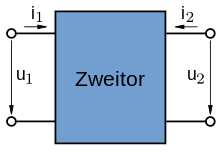
\includegraphics[width=5cm]{2Tor.png}
	\label{fig:übersicht}
\end{figure}